% !TeX spellcheck = en_GB
% A LaTeX (non-official) template for ISAE projects reports
% Copyright (C) 2014 Damien Roque
% Version: 0.2
% Author: Damien Roque <damien.roque_AT_isae.fr>

\documentclass[a4paper,12pt]{article}
\usepackage[utf8]{inputenc}
\usepackage[T1]{fontenc}
\usepackage[english]{babel} % If you write in English
\usepackage[a4paper,bindingoffset=0in,%
	left=0.8in,right=0.8in,top=1.4in,bottom=1.2in,%
	footskip=.25in]{geometry}
\usepackage{graphicx}
\graphicspath{{img/}}
%\usepackage{subfig}
\usepackage{dirtree}
\usepackage{caption, subcaption}
%\usepackage{tikz}
%\usetikzlibrary{shapes,arrows}
\usepackage{array}
\usepackage[dvipsnames,table]{xcolor}
\usepackage{tabularx}
\usepackage{longtable}                     
\usepackage{ltxtable} 
\usepackage{pgfplots}
\pgfplotsset{compat=newest}
\pgfplotsset{plot coordinates/math parser=false}
\newlength\figureheight
\newlength\figurewidth
\pgfkeys{/pgf/number format/.cd,
set decimal separator={,\!},
1000 sep={\,},
}
\renewcommand{\baselinestretch}{1.05}
\usepackage{fancyhdr}
\pagestyle{fancy}
\fancyfoot{}
\fancyhead[LE,RO]{\bfseries\thepage}
\fancyhead[RE]{\bfseries\nouppercase{\leftmark}}
\fancyhead[LO]{\bfseries\nouppercase{\rightmark}}
\setlength{\headheight}{15pt}

\let\headruleORIG\headrule
\renewcommand{\headrule}{\color{black} \headruleORIG}
\renewcommand{\headrulewidth}{1.0pt}
\usepackage{colortbl}
\arrayrulecolor{black}

\fancypagestyle{plain}{
  \fancyhead{}
  \fancyfoot[C]{\thepage}
  \renewcommand{\headrulewidth}{0pt}
}

\makeatletter
\def\@textbottom{\vskip \z@ \@plus 1pt}
\let\@texttop\relax
\makeatother

\makeatletter
\def\cleardoublepage{\clearpage\if@twoside \ifodd\c@page\else%
  \hbox{}%
  \thispagestyle{empty}%
  \newpage%
  \if@twocolumn\hbox{}\newpage\fi\fi\fi}
\makeatother

\usepackage{amsthm}
\usepackage{amssymb,amsmath,bbm}
\usepackage{array}
\usepackage{bm}
\usepackage{multirow}
\usepackage[footnote]{acronym}
\usepackage{url}
\usepackage{filecontents}
\usepackage{ifthen}
\usepackage{ifpdf}
\ifpdf
\usepackage[pdftex,backref=page]{hyperref}
\else
\usepackage[backref=page]{hyperref}
\fi
\hypersetup{%
	colorlinks=true,
	linkcolor=blue,
	citecolor=green,
	urlcolor=blue}
\usepackage{cleveref}

\newcommand*{\SET}[1]  {\ensuremath{\mathbf{#1}}}
\newcommand*{\VEC}[1]  {\ensuremath{\boldsymbol{#1}}}
\newcommand*{\FAM}[1]  {\ensuremath{\boldsymbol{#1}}}
\newcommand*{\MAT}[1]  {\ensuremath{\boldsymbol{#1}}}
\newcommand*{\OP}[1]  {\ensuremath{\mathrm{#1}}}
\newcommand*{\NORM}[1]  {\ensuremath{\left\|#1\right\|}}
\newcommand*{\DPR}[2]  {\ensuremath{\left \langle #1,#2 \right \rangle}}
\newcommand*{\calbf}[1]  {\ensuremath{\boldsymbol{\mathcal{#1}}}}
\newcommand*{\shift}[1]  {\ensuremath{\boldsymbol{#1}}}

\newcommand{\eqdef}{\stackrel{\mathrm{def}}{=}}
\newcommand{\argmax}{\operatornamewithlimits{argmax}}
\newcommand{\argmin}{\operatornamewithlimits{argmin}}
\newcommand{\ud}{\, \mathrm{d}}
\newcommand{\vect}{\text{Vect}}
\newcommand{\sinc}{\ensuremath{\mathrm{sinc}}}
\newcommand{\esp}{\ensuremath{\mathbb{E}}}
\newcommand{\hilbert}{\ensuremath{\mathcal{H}}}
\newcommand{\fourier}{\ensuremath{\mathcal{F}}}
\newcommand{\sgn}{\text{sgn}}
\newcommand{\intTT}{\int_{-T}^{T}}
\newcommand{\intT}{\int_{-\frac{T}{2}}^{\frac{T}{2}}}
\newcommand{\intinf}{\int_{-\infty}^{+\infty}}
\newcommand{\Sh}{\ensuremath{\boldsymbol{S}}}
\newcommand{\C}{\SET{C}}
\newcommand{\R}{\SET{R}}
\newcommand{\Z}{\SET{Z}}
\newcommand{\N}{\SET{N}}
\newcommand{\K}{\SET{K}}
\newcommand{\reel}{\mathcal{R}}
\newcommand{\imag}{\mathcal{I}}
\newcommand{\cmnr}{c_{m,n}^\reel}
\newcommand{\cmni}{c_{m,n}^\imag}
\newcommand{\cnr}{c_{n}^\reel}
\newcommand{\cni}{c_{n}^\imag}
\newcommand{\tproto}{g}
\newcommand{\rproto}{\check{g}}
\newcommand{\LR}{\mathcal{L}_2(\SET{R})}
\newcommand{\LZ}{\ell_2(\SET{Z})}
\newcommand{\LZI}[1]{\ell_2(\SET{#1})}
\newcommand{\LZZ}{\ell_2(\SET{Z}^2)}
\newcommand{\diag}{\operatorname{diag}}
\newcommand{\noise}{z}
\newcommand{\Noise}{Z}
\newcommand{\filtnoise}{\zeta}
\newcommand{\tp}{g}
\newcommand{\rp}{\check{g}}
\newcommand{\TP}{G}
\newcommand{\RP}{\check{G}}
\newcommand{\dmin}{d_{\mathrm{min}}}
\newcommand{\Dmin}{D_{\mathrm{min}}}
\newcommand{\Image}{\ensuremath{\text{Im}}}
\newcommand{\Span}{\ensuremath{\text{Span}}}

\renewcommand*{\backref}[1]{}
\renewcommand*{\backrefalt}[4]{%
	\ifcase #1 (Not cited.)%
	\or        (Cited on page~#2.)%
	\else      (Cited on pages~#2.)%
	\fi}

\newtheoremstyle{break}
  {11pt}{11pt}%
  {\itshape}{}%
  {\bfseries}{}%
  {\newline}{}%
\theoremstyle{break}

%\theoremstyle{definition}
\newtheorem{definition}{Définition}[section]

%\theoremstyle{definition}
\newtheorem{theoreme}{Théorème}[section]

%\theoremstyle{remark}
\newtheorem{remarque}{Remarque}[section]

%\theoremstyle{plain}
\newtheorem{propriete}{Propriété}[section]
\newtheorem{exemple}{Exemple}[section]
\definecolor{mylred}{HTML}{ffe4e1}
\definecolor{myred}{HTML}{b63e33}

\newcolumntype{x}[1]{>{\centering\arraybackslash\hspace{0pt}}p{#1}}

\parskip=5pt
%\sloppy

\begin{document}

%%%%%%%%%%%%%%%%%%
%%% First page %%%
%%%%%%%%%%%%%%%%%%

\begin{titlepage}
\thispagestyle{empty}
\begin{center}
	
%{\large University of Padua}\\[0.5cm]


\includegraphics[width=0.45\textwidth]{logo-unipd}\\[1cm]

{\large Department of Mathematics}\\[0.5cm]

{\large Computer Science Master's degree}\\[0.5cm]

{\large Course of Methods and models for combinatorial optimization a.y. 2019/20}\\[0.5cm]

%{\large Project report}\\[0.5cm]

% Title
\rule{\linewidth}{0.5mm} \\[0.4cm]
{ \huge \bfseries TSP project report \\[0.4cm] }
\rule{\linewidth}{0.5mm} \\[1.5cm]

% Author and supervisor
\noindent
\begin{minipage}{0.4\textwidth}
  \begin{flushleft} \large
    \emph{Author:}\\
    Alessandro \textsc{Zangari}
  \end{flushleft}
\end{minipage}%
\begin{minipage}{0.4\textwidth}
  \begin{flushright} \large
    \emph{Student id:} \\
    \textsc{1207247}
  \end{flushright}
\end{minipage}

\vfill

% Bottom of the page
{\today}

\end{center}
\end{titlepage}

%%%%%%%%%%%%%%%%%%%%%%%%%%%%%
%%% Non-significant pages %%%
%%%%%%%%%%%%%%%%%%%%%%%%%%%%%

%\frontmatter

%\clearpage

\begingroup
\hypersetup{colorlinks=false, linkcolor=black}
\thispagestyle{empty}
\tableofcontents
%\clearpage
\thispagestyle{empty}
\listoffigures
\thispagestyle{empty}
\listoftables
\endgroup

%%%%%%%%%%%%%%%%
%%% Abstract %%%
%%%%%%%%%%%%%%%%

\thispagestyle{empty}
\clearpage
%\vspace*{\fill}
\noindent\rule[2pt]{\textwidth}{0.5pt}\\
\thispagestyle{empty}
\section*{Abstract}
The following report documents the course project, which demanded the development of two algorithms to solve the Travelling Salesman Problem. The first algorithm uses the C IBM CPLEX API to obtain the exact solution. The second algorithm is an heuristic method, whose functioning is inspired by the Lin-Keringhan heuristic.

%%%%%%%%%%%%%%%%%%%%%%%%%%%%%%%%%%%%%%%%%%%%
%%% Content of the report and references %%%
%%%%%%%%%%%%%%%%%%%%%%%%%%%%%%%%%%%%%%%%%%%%

%\mainmatter
\pagestyle{fancy}

\cleardoublepage

% !TeX spellcheck = en_GB
% !TeX root = memoco-report.tex

\section{Introduction}
\label{chap:introduction}

\subsection{Description of the problem}
The task of the exercise was to develop two algorithms capable of solving the Travelling Salesman Problem (TSP), specialized to the domain of drilling holes in electric panels. Given a sequence of holes to be drilled in an electric panel, the algorithms should be used to find a sequence of holes that minimizes the cost of drilling the whole panel, where the costs are given by the euclidean distances between holes. For simplicity it is assumed that the cost of drilling every hole can be ignored.\\ 
The first algorithm implements an exact methods using the IBM CPLEX optimization suite. The second algorithm is an approximated heuristic, inspired by the Lin-Kernighan algorithm \cite{LinK73}. Some implementation details has been taken from \cite{ImplemLK}. \\
Both algorithms have been tested on synthetic instances produced taking into account the applicative domain. The two algorithms are described in the following pages, and tests and results are reported in the last sections.

\subsection{Description of provided material}
%\minitoc
The delivered material includes all the produced code and everything necessary to run the program.
The provided archive comes with the following structure:
\renewcommand*\DTstylecomment{\rmfamily\color{blue}\textit}
\dirtree{%
	.1 /.
	.2 bin/\DTcomment{Binary files folder}.
	.2 build/\DTcomment{Build files folder}.
	.2 files/\DTcomment{Logs folder}.
	.2 instances/\DTcomment{Contains csv files to load}.
	.2 plots/.
	.2 src/.
	.3 utils/.
	.4 cpxmacro.hpp.
	.4 params.hpp.
	.4 python\_adapter.hpp\DTcomment{Wrapper class for Python embedding}.
	.4 variadic\_table.hpp\DTcomment{Library to print tables}.
	.4 yaml\_parser.hpp\DTcomment{Parser for the configuration file}.
	.3 calibrate.cpp\DTcomment{Calibration script}.
	.3 config.yml.
	.3 CPLEX.cpp.
	.3 CPLEX.hpp.
	.3 LK.cpp.
	.3 LK.hpp.
	.3 main.cpp\DTcomment{Program main}.
	.3 Pair.cpp.
	.3 Pair.hpp.
	.3 plot\_script.py\DTcomment{Script to plot with Python}.
	.3 test.cpp\DTcomment{Test script}.
	.3 Tour.cpp.
	.3 Tour.hpp.
	.3 TSPinstance.cpp.
	.3 TSPinstance.hpp.
	.3 TSPsolution.cpp.
	.3 TSPsolution.hpp.
	.3 utilities.cpp.
	.3 utilities.hpp.
}

\subsubsection{How to run}
The program has the following dependences:
\begin{itemize}
	\setlength\itemsep{0.03em}
	\item \texttt{g++ 7} or higher;
	\item \texttt{IBM ILOG CPLEX Optimization Studio 12.8} or higher;
	\item \texttt{Python 2.7}.
\end{itemize}

To test the program, some instances should be generated or imported by placing them in the \texttt{instances/} folder. Some files are already provided in this folder to launch some tests. To generate new instances set \texttt{generate\_instances: true} in the \texttt{config.yml} file, and the other parameters as desired. If \texttt{N\_min = 20, N\_incr = 5, N\_max = 30}, three \texttt{csv} files containing the coordinates of every point will be generated, with size 20, 25 and 30 respectively, and will be placed in the instances folder. After that it is possible to run the exact method or the heuristic on these instances. To do that, add to the list in \texttt{instances\_to\_read} the filename (without extension) of the files that should be read and set \texttt{solve\_heur} and \texttt{solve\_cplex} as desired. Some reasonable parameters for the heuristic are already set, but it is possible to change them if necessary. A description of these specific parameters is provided in \cref{ssec:hyperpar}.
The script can then be run from a Linux environment with \texttt{make \&\& ./bin/main}. The algorithm writes its output in file \texttt{solLK.txt} and \texttt{solCPLEX.txt} under the \texttt{files/} folder. When solving more than one problem, these files can also be checked while the program is running to monitor its execution. Additionally running the heuristic also produces an image of the final solution and places it in folder \texttt{plots/}. Furthermore, running both CPLEX and the heuristic together will produce plots with a comparison of the execution times and error values in the same folder. \\

\subsection{Development environment}
The specifics of the machine used for development, calibration and test of the program are listed in \cref{tab:maspecs}.
\begin{table}[H]
	\caption{Hardware and software specifics}
	\label{tab:maspecs}
	\centering
	\begin{tabular}[t]{ll}
		\rowcolor[HTML]{EFEFEF}
		\textbf{Specific} & \textbf{Value} \\
		OS       & Ubuntu 18.04.4 LTS 64 bit	   \\
		Processor & Intel Core i7-7500U 2.70GHz $\times$ 4     \\
		Main memory  & 16 GB  
	\end{tabular}
\end{table}

\section{Dataset generation}
\label{sec:datasetgen}
In order to test the two algorithms, a procedure to build a synthetic dataset of different sizes has been provided.\\ 
The procedure to generate the TSP instances receives as an input a number $N$ of points (which symbolises holes) and generates $N$ pairs representing the coordinates in space of the points on a $N\times N$ square canvas. These points are distributed in a way to resemble the regularity usually found in the disposition of holes in electric panels.\\ 
To do this the procedure draws some regular polygons with up to $10$ sides. Each polygon is generated independently and may overlap with the others, creating not perfectly regular shapes, but neither a completely random point distribution. An example of such an instance is shown in \cref{fig:dataexample}. All this operations, as well as the function to load already generated instances from \texttt{csv} files, are implemented in \texttt{TSPinstance.cpp}.

\begin{figure}[h]
	\centering
	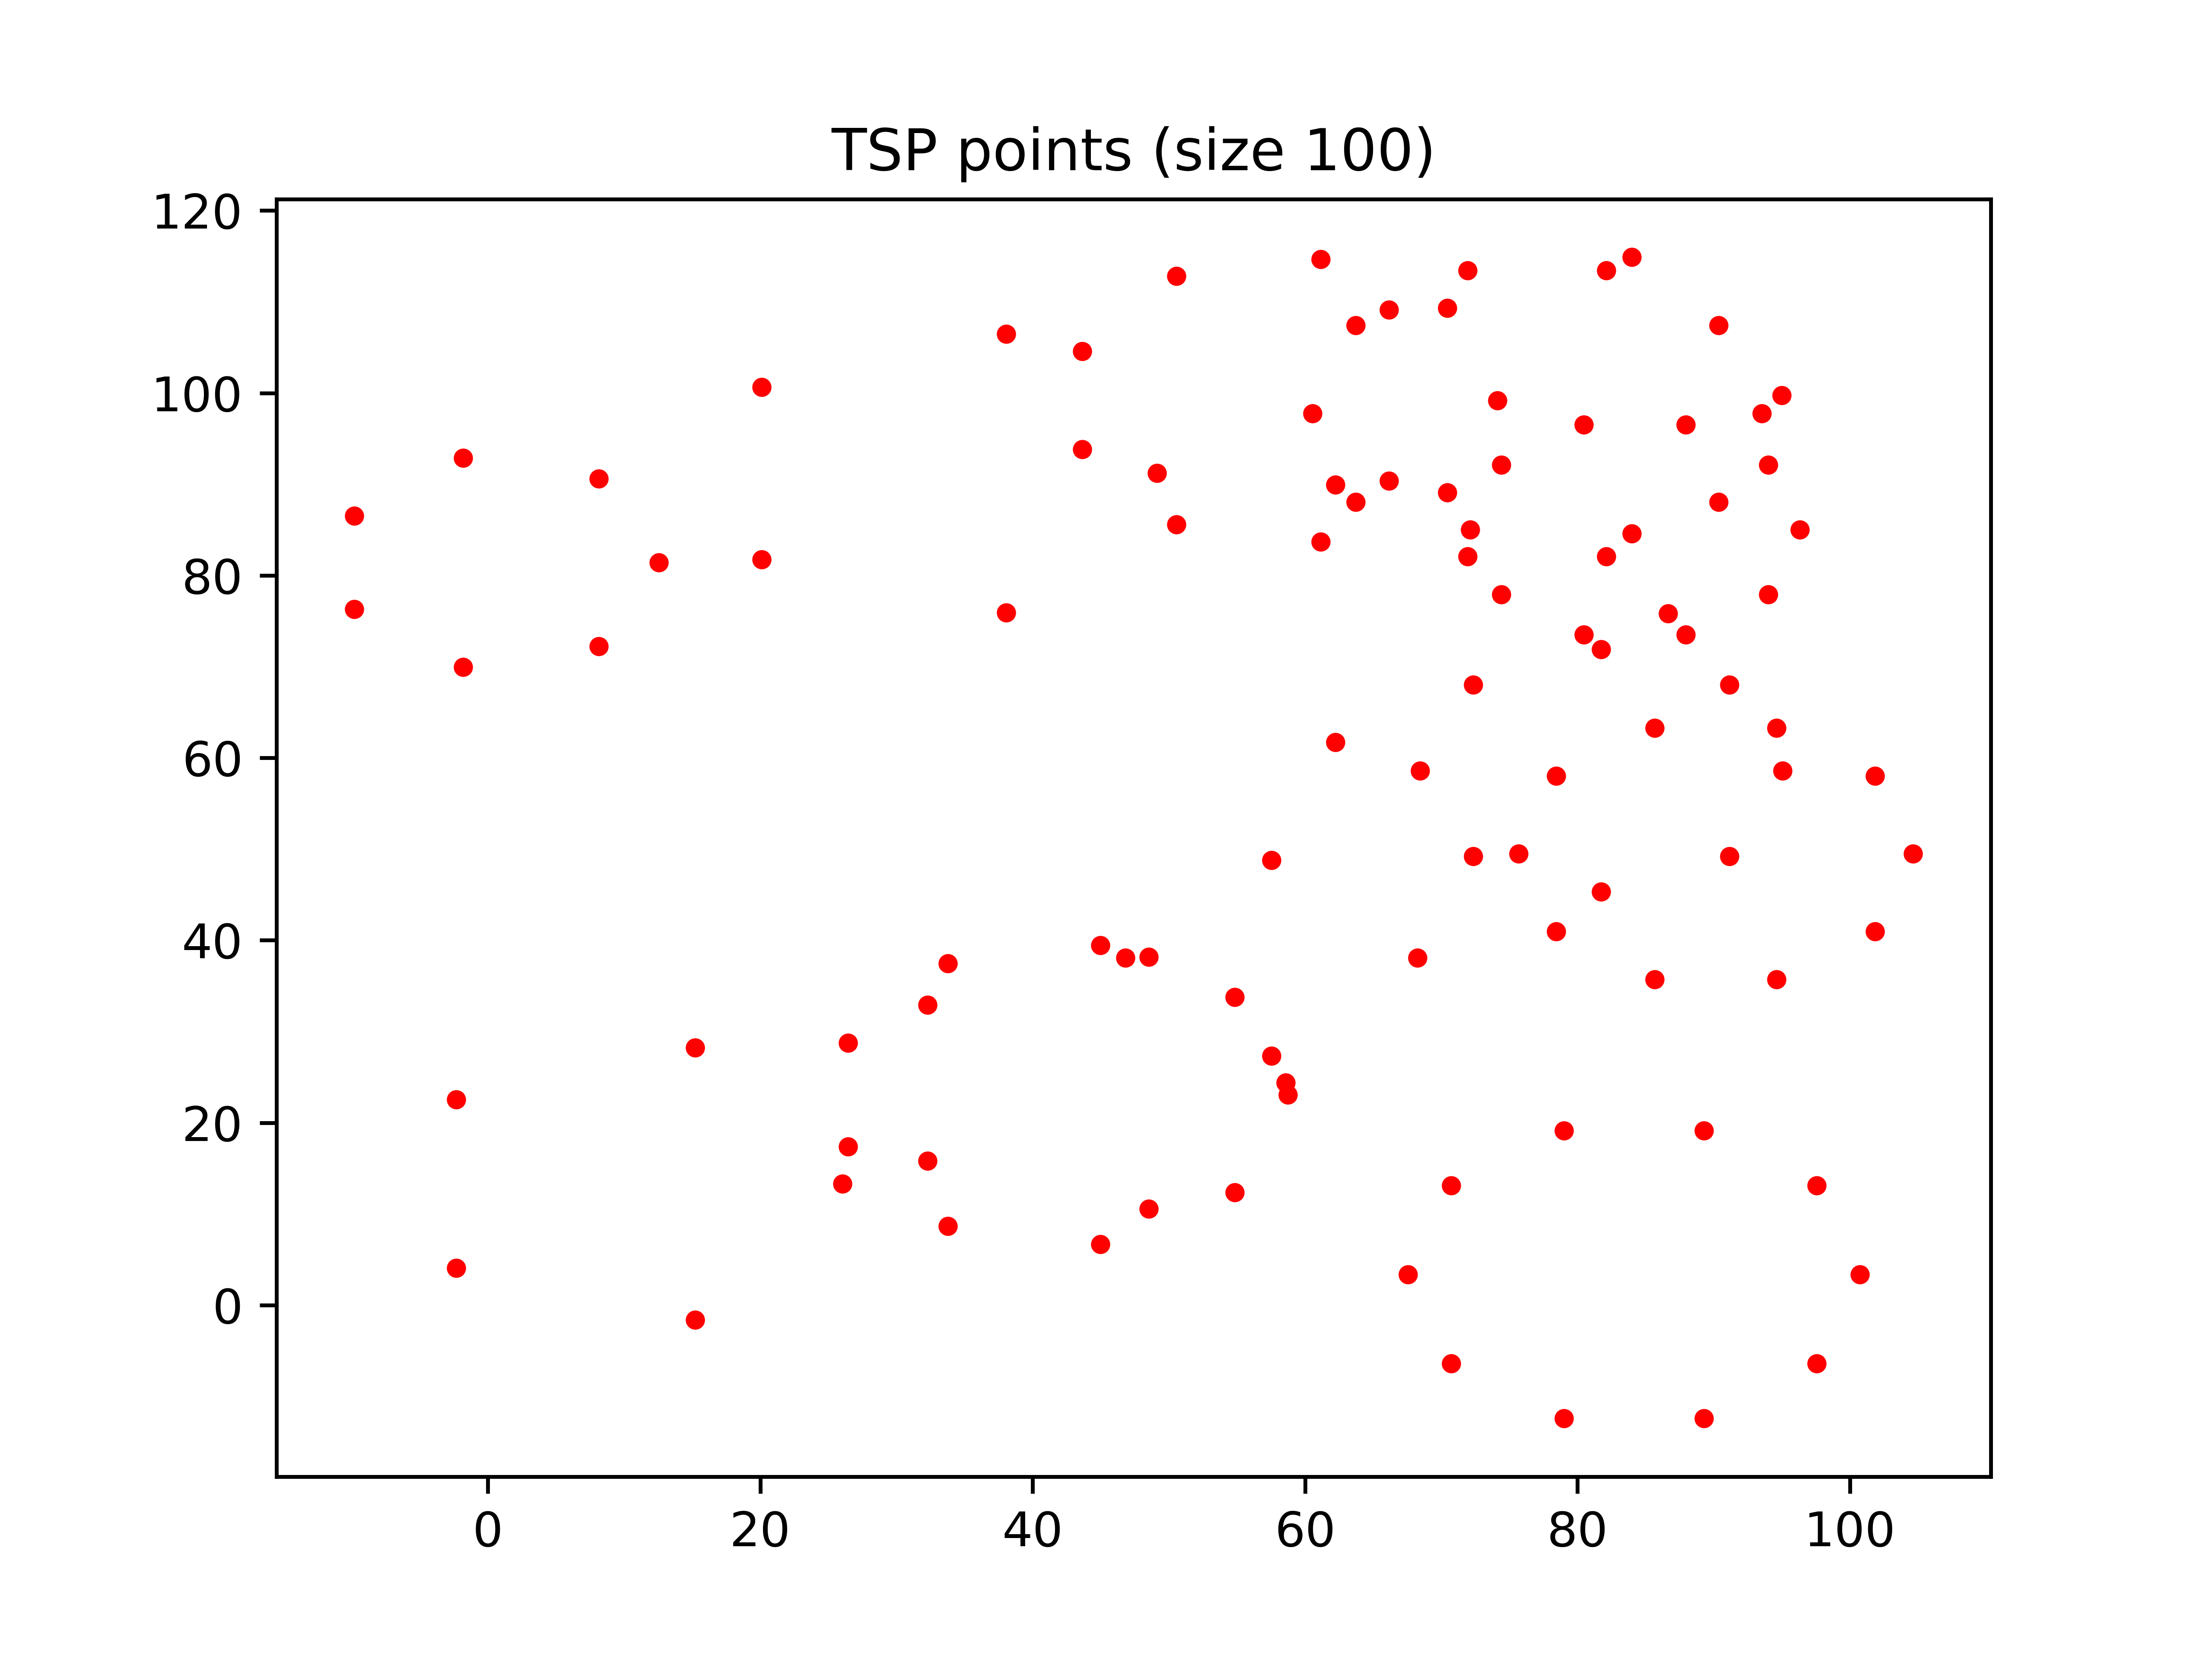
\includegraphics[width=13cm]{path_100}
	\caption{A generated instance of with size N = 100}
	\label{fig:dataexample}
\end{figure}



\section{Exact method}
\label{chap:cplexm}
\subsection{Description}

%\begin{figure}[htp]
%  \centering
%  \includegraphics[width=4cm]{images/bitmap_image}
%  \caption{Exemple d'image au format JPG.}
%  \label{fig:une-autre-image}
%\end{figure}

\section{Heuristic method}
\label{chap:heuris}
\subsection{Description}

\subsection{Hyperparameters}

\subsubsection{Calibration}




%%% Local Variables: 
%%% mode: latex
%%% TeX-master: "isae-report-template"
%%% End: 
\section{Tests and results}
\label{sec:unchapitre}

%%% Local Variables: 
%%% mode: latex
%%% TeX-master: "isae-report-template"
%%% End: 
% !TeX spellcheck = en_GB
% !TeX root = memoco-report.tex
\section{Conclusions}
\label{sec:conclusion}
The implemented heuristic can be expected to find very good (if not optimal) solutions for problem of small size and outperforms the exact algorithm in every conducted test. For problem of size greater than 40 the gap in running time between the two algorithms becomes very large, several minutes for the exact method and a few seconds for the heuristic that will likely find the optimal solution anyway.\\
Tests on TSPLIB drilling problems suggests encouraging performances on non trivial sizes, even though the runtime grows, and some parameters may be adjusted to favour execution time at the expense of solution quality.
For the optimization of the drilling paths over electric boards, the heuristic method seems the preferable choice even for small boards, since it often finds the optimal solution with a reasonable number of restarts. \\
Performance on instances with thousands of holes remains to be tested. Literature suggests that by refining this algorithm some more, good results could be achieved.
    
\subsection{Possible improvements}
The Lin-Keringhan local search algorithm received many reformulations, adaptations and improvements since its original publication that can be found in literature, so many of these ideas could be exploited to improve the hereby described algorithm.\\
A first improvement could relate to the tour representation, since there are better data structures to represent an Hamiltonian cycle. For example \cite{GLOVER1996223} proposed \textit{ejection chains}, structures that would allow for a fast (constant time) lookup when deciding if breaking a new edge allows a feasible tour or not. This would improve the efficiency and efficacy of the neighbourhood function and thus of the entire algorithm. \\
Some more work could be done to choose what to do when an already found solution is encountered for the second time, as already suggested in \cref{sssec:checkout}.\\ Additionally the intensification strategy could be refined by using a probabilistic approach to give some more flexibility.\\
Finally a speed-up could be achieved by exploiting multithreading to launch more executions concurrently. At the moment, every restart shares with the previous executions the set of solutions found, in order to avoid converging to the same solution again, so parallelization is not feasible, but this strategy could be reviewed.\\

%%% Local Variables: 
%%% mode: latex
%%% TeX-master: "isae-report-template"
%%% End: 



\appendix

\bibliographystyle{alpha}
\bibliography{references}

\clearpage

\end{document}